Chazelle \cite{C2000} proposed in 2000 a new algorithm which solves the minimum spanning tree problem.  He has proven that the algorithm runs in $O(m\alpha(m,n))$ time. It has not been improved on since by any other algorithm with known complexity.

\section{Idea and pseudocode}
The main idea of the algorithm is to partition a graph into smaller subgraphs for which we compute the minimum spanning trees recursively. In order to make it fast the smaller minimum spanning trees together form a spanning tree that is not necessarily minimal. However in the process some edges are proven not to be in the MST and other's have to be reprocessed in a final recursive call.

There are several ideas that work together in this algorithm and this section is devoted to explaining them.

\subsection{Contractible subgraphs}

 It is important to have a certain mindset when considering the MST problem -- that is, one has to think about it in terms of edge contractions. In particular, let us reacall an importanat duality between to properties:
 \begin{itemize}
     \item cut property (\Cref{cut-property}) -- allows us to prove that edge is in the MST and can be contracted.
     \item cycle property (\Cref{cycle-property}) -- allows us to prove that edge is outside of the MST and can be discarded.
 \end{itemize}
These properties are crucial both for the construction of algorithms and for the proofs of certain properties like strong contractibility -- which we will consider now. 

\begin{definition} [Contractible subgraph \cite{C2000}]
A connected induced subgraph $H \subseteq G$ is contractible if and only if $MST(H) \subseteq MST(G)$.
\end{definition}

The notion of contractible subgraphs is helpful when creating divide and conquer algorithms for the MST problem as we shall see below.

Let's say we have a partition of the vertices of a graph $G$ into sets {$V_1, V_2, ..., V_k$} and corresponding induced subgraphs {$G_1, G_2, ..., G_k$}. Denote $G'$ as a graph $G$ after contracting each of the $V_i$ sets of vertices. Now we can see that thanks to the definition of contractible subgraphs we have that
\begin{equation}
MST(G) = \left(\bigcup\limits_{i=1}^{k} MST(V_i)\right) \cup MST(G').
\end{equation}
 
Having that we could recursively apply our MST algorithm and just sum the results.

While contractibility is extremely useful, it is a global property. That is, it depends on the $MST(G)$. Thus proving it from the definition requires computing the $MST(G)$ first.

\begin{definition} [Strongly contractible subgraph]
A connected induced subgraph $H \subseteq G$ is strongly contractible if and only if for all $e,f \in E(G)$ with exactly one endpoint in $H$, there exists path in $H$ which connects $e$ and $f$ and no edge along this path exceeds the cost of both $e$ and $f$.
\end{definition}

\begin{lemma}
If a subgraph $H$of $G$ is strongly contractible then it is contractible.    
\end{lemma}

\begin{proof}
Let's assume $H$ is not contractible, thus $MST(G)\ \cap\ H$ has to have multiple connected components. Let's take a shortest path in $MST(G)$ that connects these components. It is the shortest so it cannot have edges in $H$, let $e, f$ be the first and last edge i.e. the edges which connect $H$ to the $G/H$. 

But the subgraph $H$ is connected and strongly contractible, so there is a path that completes the cycle and lies fully inside $H$ and has all of the edge costs smaller than $\max\{c(e), c(f)\}$. So the largest edge on this cycle lies outside the path in $H$, and by the cycle property it cannot be in the $MST(G)$ -- a contradiction.     
\end{proof}

The notion of strongly contractible subgraphs is local. It allows us to certify contractibility of a given subgraph by looking only at it and its neighborhood.

\subsection{$T$-hierarchy}
\subsubsection{Borůvka}
To introduce the concept of $T$-hierarchy let's first consider Borůvka's algorithm:

\begin{algorithm}[H]
\caption{Borůvka’s Algorithm}
\label{bor}
\begin{algorithmic}[1]
\Function{Boruvka}{$G \colon \texttt{Graph}$}
    \State $F \gets \emptyset$ 
    \While{$|E| > 0$}
        \State $F \gets F\ \cup\ $ \Call{Boruvka-step}{$G$}
    \EndWhile
    \State \Return $F$
\EndFunction
\end{algorithmic}
\end{algorithm}

\begin{algorithm}[H]
\caption{\textsc{Boruvka-step}}
\label{bor-step}
\begin{algorithmic}[1]
\Function{Boruvka-step}{$G\colon \texttt{Graph}$}
    \State $F \gets \emptyset$
    \State $marked \gets \emptyset$
    \For{$v \in V(G)$}
        \State $e \gets \arg\min{\{c(e)\colon e \in E(v)\}}$
        \State $marked \gets marked \cup \{e\}$
    \EndFor
    \For{$e \in marked$}
        \State \Call{contract}{$G, e$}
        \State $F$\Call{.insert}{$e$}
    \EndFor
    \State \Return $F$
\EndFunction
\end{algorithmic}
\end{algorithm}
\FloatBarrier
Let's consider what happens to a connected graph $G$ during the \Cref{bor-step}. Let $n, m$ be number of vertices and edges in $G$. We can see that the number of vertices in the resultant graph will be at most $\frac{n}{2}$, i.e. it drops by a factor of $2$. So the \Cref{bor} calls \Cref{bor-step} only $O(\log{n})$ times. 

 Unfortunately the number of edges $m$ doesn't always drop by a multiplicative factor. In the worst case only $\frac{n}{2}$ edges will be contracted. Given the fact that \textsc{Boruvka-step} can be performed in $O(n + m)$ time gives the total running time $O(m\log{n})$. 
 
 Consider what would happen if the number of edges decreased in every iteration by a multiplicative factor $q$, then the whole algorithm would run in time \begin{equation*}
     \left(n + m\right) + \left(\frac{n}{2} + qm\right) + \left(\frac{n}{4} + q^2m\right) ... \leq 2n + \frac{1}{1-q} m = O(n + m).
 \end{equation*}

So if we found a way to remove a factor of edges in linear or almost linear time, then we could also perform a single \Cref{bor-step} in linear time to also decrease the number of vertices by some factor and have a routine that works in linear or slightly larger time.

\subsubsection{Borůvka hierarchy}
Consider the sequence of graphs produced during consecutive \textsc{Boruvka-step} invocations. Each consecutive graph is a minor of the previous one, as \textsc{Boruvka-step} only performs edge contractions. Being a minor is a transitive property so a graph obtained after any number of \Cref{bor-step} will be a minor of every previous one.

Now looking at just one \Cref{bor-step} we can also think about it as of identifying multiple vertices as one, in this spirit we could create a forest which has two sets of vertices -- first set corresponds to vertices in original graph and the second one has vertices from the resultant minor. We can connect vertices $v$ from the first set and $w$ from the second set if $w$ was created by contracting $v$ and some other vertices. See \Cref{fig-mst} and \Cref{fig-forest}.

\begin{figure}[ht!]
    \centering
    \begin{tikzpicture}[
        vertex/.style={circle, draw, minimum size=8mm},
        edge/.style={draw, thick}
    ]
        % Nodes
        \node[vertex] (1) {1};
        \node[vertex, right=2cm of 1] (2) {2};
        \node[vertex, below=2cm of 1] (3) {3};
        \node[vertex, right=2cm of 3] (4) {4};

        % Edges
        \draw[edge, red] (1) -- (2) node[midway, above] {\small 1};
        \draw[edge] (1) -- (3) node[midway, left]  {\small 7};
        \draw[edge] (2) -- (3) node[midway, right] {\small 5};
        \draw[edge, red] (3) -- (4) node[midway, below] {\small 2};
    \end{tikzpicture}
    \caption{Example graph. Red edges are contracted in the first run of \Cref{bor-step}.}
    \label{fig-mst}
\end{figure}

\begin{figure}[ht!]
    \centering
    \begin{tikzpicture}[
        vertex/.style={circle, draw, minimum size=12mm},
        edge/.style={draw, thick}
    ]
        % Super-nodes
        \node[vertex] (A) {1,2};
        \node[vertex, right=4cm of A] (B) {3,4};

        % Edge
        \draw[edge, red] (A) -- (B) node[midway, above] {\small 5};
    \end{tikzpicture}
    \caption{The example graph minor after the \Cref{bor-step} -- also the $C_{1,2,3,4}$ graph.}
\end{figure}

\begin{figure}[ht!]
\centering
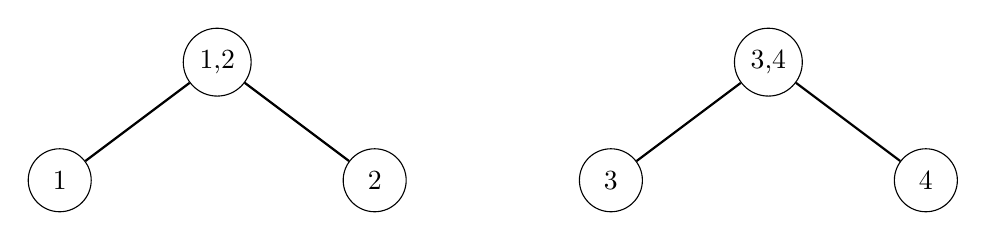
\begin{tikzpicture}[
    level distance=1.5cm,
    every node/.style={circle, draw, minimum size=8mm},
    edge from parent/.style={draw, thick}
]
% First tree
\node {1,2}
    child[sibling distance=4cm] { node {1} }
    child[sibling distance=4cm] { node {2} };

% Second tree (shifted to the right)
\node at (7,0) {3,4}
    child[sibling distance=4cm] { node {3} }
    child[sibling distance=4cm] { node {4} };
\end{tikzpicture}
\caption{Forest corresponding to a single iteration of \Cref{bor-step}.}
\label{fig-forest}
\end{figure}



If we extend that forest by adding sets of vertices corresponding to minor's in each consecutive \Cref{bor-step} iteration we will get a tree $T$, which root represents a contraction of all vertices into a single node. Each layer below it corresponds to the minor from the previous iteration, and leafs of this tree $T$ are just the vertices of the original graph $G$ for which we want to find the minimum spanning tree. See \Cref{t-h} below.

\begin{figure}[H]
\centering
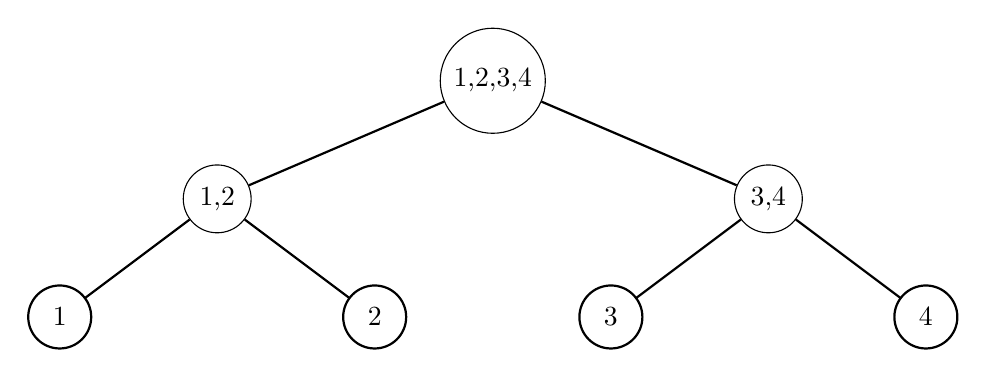
\begin{tikzpicture}[
    level distance=1.5cm,
    every node/.style={circle, draw, minimum size=8mm},
    edge from parent/.style={draw, thick}
]
    % Root
    \node {1,2,3,4}
        child[sibling distance=7cm] { node {1,2}
            child[sibling distance=4cm] { node {1} }
            child[sibling distance=4cm] { node {2} }
        }
        child[sibling distance=7cm] { node {3,4}
            child[sibling distance=4cm] { node {3} }
            child[sibling distance=4cm] { node {4} }
        };
\end{tikzpicture}
\caption{$T$-hierarchy constructed by the \Cref{bor}.}
\label{t-h}
\end{figure}

\begin{figure}[H]
    \centering
    \begin{tikzpicture}[
        vertex/.style={circle, draw, minimum size=12mm},
        edge/.style={draw, thick}
    ]
        % Super-nodes
        \node[vertex] (A) {1};
        \node[vertex, right=4cm of A] (B) {2};

        % Edge
        \draw[edge] (A) -- (B) node[midway, above] {\small 1};
    \end{tikzpicture}
    \caption{The $C_{1,2}$ graph}
\end{figure}
\FloatBarrier

\begin{definition}[$T$-hierarchy]
    $T$-hierarchy is a rooted tree $T$, whose leaves correspond to the vertices of a given graph $G$ and the internal nodes represent contractions of all of the leaves below them.  
\end{definition}
In particular root corresponds to the contraction of the whole graph $G$ and a subtree of $T$ corresponds to a minor of the graph $G$.

\begin{definition}[$z_i \texttt{ and } C_{z_i}$]
We introduce the notation that $z_i$ is an internal node of the tree $T$ and $C_{z_i}$ is a graph whose vertices are the children of $z_i$. The edge between vertices $u$ and $v$ in this graph corresponds to the smallest edge (if it exists) joining sets of vertices of $G$ -- the leaves below $u$ and $v$ in the $T$-hierarchy respectively.   
\end{definition}

Now the $T$-hierarchy constructed by the Borůvka's algorithm has an important property. If you look at any node in the hierarchy its correspondent set of vertices of $G$ induces a contractible subgraph in $G$. This property follows directly from the fact that the hierarchy was created by contracting the edges which belong to the $MST(G)$.

If we were given a $T$-hierarchy with this property, we could compute the minimum spanning tree using the divide and conquer method with the following lemma:
\begin{lemma}[$MST$ construction using $T$-hierarchy]
Given a graph $G$ and corresponding $T$-hierarchy such that for every $z\in V(T)$ its $C_{z}$ is contractible we can find the $MST(G)$ using the following identity:
\begin{equation*}
    MST(G) = \bigcup\limits_{z\in T}MST(C_z).
\end{equation*}
\label{divide-conq}
\end{lemma}
\begin{proof}
    We repeatedly apply (2.1) until the $G'$ is fully contracted. Consider what happens after one application of (2.1) to the original graph $G$ and a partition into the contractible subgraphs defined by the bottom layer of $T$ ($z$ such that all of $z$'s children are leaves). 
    
    For example for \Cref{t-h}, after the first application of (2.1) we are left with a $G'$ and its $T$-hierarchy $T'$ which was obtained from $T$ by pruning all of the leaves $1, 2, 3$ and $4$. 
\end{proof}

\subsection{Reverse the construction schedule}
One of the main ideas behind the algorithm is to reverse the MST construction schedule. First we could create a hierarchy $T$ such that each layer represents a partition of the graph $G$ into contractible subgraphs. Then we would calculate the $MST(G)$ recursively using the \Cref{divide-conq}.

\subsubsection{Corruption}
Nevertheless, calculating the $T$-hierarchy proves to be a difficult task. To make this step fast Chazelle decided to loosen the requirements put on the $T$-hierarchy. During its creation some edges will become corrupted, that is their weight will be purposefully made higher then original. The resultant $T$-hierarchy will have its internal nodes contractible, but in terms of the \textbf{working cost} of the edges and not counting the \textbf{discarded} edges (both notions will be defined later). 

It is important to mention that all of the \textbf{discarded} edges and also the edges for which the \textbf{working cost} is different than their original cost will be reprocessed later with their costs reverted back to the original.

\begin{remark}[Edge corruption]
    Each edge of the graph $G$ has its original cost and current cost associated with it. The current cost can change during a construction of $T$, but will never be lower than the original cost. We call edges \textbf{corrupted} when their current and original costs differ.

    %When referring to the current cost of an edge, unless explicitly stated otherwise, we refer to the current cost at the moment when the $T$ has been constructed and the costs are now frozen.%
\end{remark}

\subsubsection{Prim}
In order to understand why and how the corruption happens and what are the working costs of the edges referred to in the previous subsection we need to first understand how the $T$-hierarchy is built. 

Let's first consider Prim's algorithm as it will be the basis for the $T$-hierarchy construction. We can think about it as picking a vertex $v$ and sequentially contracting entire graph to it edge by edge. It also can be thought of as a Dijkstra analogue: there are visited and unvisited nodes and we always visit the closest one, but not the closest one to the origin $v$ like in Dijkstra.

\begin{algorithm}[H]
\caption{Prim's Algorithm}
\begin{algorithmic}[1]
\Function{Prim}{$G\colon \texttt{Graph}$}
    \State $v \gets$ \Call{pick-any-vertex}{$G$}
    \State $F \gets \emptyset$
    \While{$E(G) \neq \emptyset$}
        \State $e \gets$ \Call{smallest-edge-adjacent-to}{$v$}
        \State \Call{contract-edge}{$e, G$}  \Comment{Contracts other vertex $u$ into $v$}
        \State $F \gets F \cup \{e\}$
    \EndWhile
    \State \Return $F$
\EndFunction
\end{algorithmic}
\end{algorithm}
\FloatBarrier

\subsubsection{Building the $T$-hierarchy}
The Prim's algorithm does not care about the already visited vertices: when a vertex $v$ is processed its edges are pushed on a priority queue and the vertex can be forgotten of.

To build the $T$-hierarchy we will perform a Prim's algorithm but with two important modifications:
\begin{itemize}
    \item we maintain a structure on the visited vertices -- this structure is the $T$-hierarchy being built.
    \item as a priority queue we will use soft heaps, a heap-like data structure devised by Chazelle.
\end{itemize}

The exact construction schedule and soft heaps will be discussed thoroughly later. For the purpose of this introduction let us mention their most important properties:

\begin{itemize}
    \item Soft heaps are responsible for the edge corruption.
    \item $T$-hierarchy is created \textbf{bottom-up} -- when a $C_z$ is assembled all of its children are constructed too and the current costs of edges inside them are frozen. When the $C_z$ has been constructed it gets contracted to a vertex and put inside its parent.
    \item In the process of construction some edges are \textbf{discarded} -- these edges were necessarily bad.
\end{itemize}

Let us finally introduce the crucial auxiliary notions for this algorithm:
\begin{definition}[Border edge]
    During the Prim's algorithm if the edge joins a visited and an unvisited node, then its a \textbf{border edge}.
\end{definition}

In the Chazelle's algorithm context during the construction of $T$-hierarchy we maintain a structure on visited nodes, that is, the $C_z$ graphs. We use the same name border edge for the edges joining visited and unvisited vertices. We also say that a border edge $\{u, v\}$ joins a $C_z$ to an unvisited vertex $v$ when the visited vertex $u$ is under the $z$ node in the $T$-hierarchy.

\begin{definition}[Bad edge]
    A border edge $e$ becomes bad if it is corrupted and has one endpoint in a current $C_z$ in the moment of its contraction.
\end{definition}
    We will sometimes reset the current costs of the edges, but once the edge becomes bad it always remains bad, even after the reset.


\begin{definition}[Working cost]
    Working cost of an edge $e$ is its current cost if it is bad, otherwise it is its original cost.
\end{definition}

\subsubsection{Soft heap}
Soft heap is a minimum heap devised by Chazelle, which is a workhorse for the algorithm. It breaks the traditional $O(\log{n})$ bound for heaps for all of its operations, but at the cost of corruption: some elements may have their keys increased. 

Each element inserted into the soft heaps has its original key, and also a ckey - they are equal in the beginning. The soft heap maintains an ordering using the ckeys and ckeys cannot be lower then keys. 

Soft heap allows for \texttt{make-heap}, \texttt{insert}, \texttt{meld}, \texttt{pop-min} and \texttt{delete} operations. Each of them runs in $O(1)$ amortized time, but for the \texttt{insert} operation which runs in $O(\log{\frac{1}{\epsilon}})$ amortized time. The $\epsilon$ parameter is set in the \texttt{make-heap}. 

Soft heap maintains an invariant that there are at most $\epsilon n$ corrupted elements on the heap, where $n$ is the number of inserted elements -- not to confuse with the number of elements currently stored in the heap.

\subsection{Pseudocodes}
\begin{algorithm}
\caption{Recursive MST Algorithm}
\begin{algorithmic}[1]
\Function{mst}{$G \colon \texttt{Graph}, \ t \colon \texttt{int}$}
    \If{$t = 1 \ \lor\ n = O(1)$} 
        \State \Return \Call{Boruvka}{$G$} \Comment{STEP 1}
    \EndIf
    \State $G_0, F_0 \gets$ \Call{Boruvka-steps}{$G, c$} \Comment{STEP 2}
    \State $T, B \gets$ \Call{construct-$T$-hierarchy}{$G_0$} \Comment{STEP 3}
    \State $F \gets \bigcup_{C_z \in T} \Call{mst}{C_z / B, \ t-1}$ \Comment{STEP 4}
    \State \Return $F_0 + \Call{mst}{F + B, \ t}$ \Comment{STEP 5}
\EndFunction
\end{algorithmic}
\label{cmst}
\end{algorithm}

\Cref{cmst} presents a basic pseudocode for the whole algorithm. It takes a graph $G$ and a number $t$ as inputs and returns $MST(G)$. The parameter $t$ is used in creation of $T$-hierarchy for tuning the recursion so that we have the double induction necessary for the complexity bound involving the inverse Ackermann function.
\begin{itemize}
    \item \textbf{STEP 1} This is the base case:  we just run the \Cref{bor} if the graph is small enough or $t = 1$. As the algorithm is recursive we need a base case.
    \item \textbf{STEP 2} We apply $c$ consecutive \textsc{Boruvka-step}s to the graph $G$ and return the resultant minor $G_0$ and the forest of contracted edges $F_0$.
    \item \textbf{STEP 3} This step is the hardest and contains most of the actual algorithm. Pseudocode and its analysis is provided below.
    \item \textbf{STEP 4} We recursively call \Cref{cmst} on $C_z$'s of all the internal nodes of $T$-hierarchy with bad edges removed from them. We collect the returned trees into a forest $F$.
    \item \textbf{STEP 5} We recursively call \Cref{cmst} on a graph created from bad edges $B$ and forest $F$ as we need to reprocess the bad edges. 
\end{itemize}

Let's get back to the most important part: the construction of $T$-hierarchy. Here is the pseudocode:
\begin{algorithm}[H]
\caption{$T$-hierarchy construction}
\begin{algorithmic}[1]
\Function{construct-$T$-hierarchy}{$G_0 \colon \texttt{Graph}$}
    \State \texttt{Cz} $\gets \emptyset$
    \State \texttt{H} $\gets \emptyset$ \Comment{set of soft heaps}
    \State \texttt{B} $\gets \emptyset$ \Comment{set of bad edges}
    \State \texttt{min-links} $\gets \emptyset$
    \State \Call{pick-starting-vertex}{}
    \While{ \Call{edges-on-heaps}{}}
        \If{\Call{met-desired-size}{}}
            \State \Call{retraction}{}
        \Else
            \State $e \gets$ \texttt{H}.\Call{pop-min}{}
            \If{\Call{need-fusion}{}}
                \State \Call{fusion}{}
            \EndIf
            \State \Call{extension}{}
        \EndIf
    \EndWhile
    \While{ \texttt{Cz}.\Call{length}{} > 1}
        \State \Call{retraction}{}
    \EndWhile
    \State \Return \texttt{Cz[1]}, \texttt{B}
\EndFunction
\end{algorithmic}
\label{tconstr}
\end{algorithm}

\begin{remark}
    All of the functions in the pseudocode above have the access to the state variables defined at the beginning. Thus, they were omitted from the function calls as they would clutter the pseudocode.
\end{remark}

As stated previously, the $T$-hierarchy construction mimics the Prim's algorithm: in each iteration of the loop we pop the smallest edge from the heaps and process it. 

Let's first consider the desired properties of $T$:
\begin{itemize}
    \item each $C_z$ has to be strongly contractible in terms of working costs and ignoring discarded edges,
    \item each $C_z$ has a desired size which it should attain before being contracted -- however, the exact sizing is only important for the runtime complexity analysis and will be discussed there.
\end{itemize}

Let's consider the variables used in \Cref{tconstr}.
\begin{itemize}
    \item \texttt{Cz} -- Is a stack of graphs which represent $C_z$'s \textbf{under construction} -- the so called active path. At the bottom of the stack lies the $C_{z_{root}}$ which corresponds to the root of $T$. Each consecutive stack item corresponds to the chld in $T$ of the previous one.   
    We use the notation $C_{z_1}, C_{z_2} ...C_{z_k}$ to enumerate all of the $C_z$ under construction.
    \item \texttt{H} is a minimum heap containing all of the border edges. For the complexity reasons (discussed later) it has to be a 2-dimensional array of soft heaps: if the active path is $C_{z_1}, C_{z_2} ...C_{z_k}$ then we have a $\texttt{H[i][j]} \text{ for all } i,j \in \{0, 1,..., k\}, i \leq j$.
    \item \texttt{B} -- a graph of the bad edges.
\end{itemize}

In order not to produce to many bad edges and enforce contractibility of the $C_z$'s following invariants will be maintained during the construction of the $T$-hierarchy.

\begin{invariant}[\cite{C2000}]
We keep an edge called a chain-link joining $C_{z_i}$ and $C_{z_{i+1}}$ for all $i \in \{1, 2, ..., k - 1\}$. Its current cost is:
\begin{enumerate}
    \item[(i)] at most that of any border edge incident to $C_{z_1} \cup \dots \cup C_{z_i}$
    \item[(ii)] less than the working cost of any edge joining 2 distinct $C_{z_j}$ with $j \leq i$
\end{enumerate}
\label{i1}
\end{invariant} 
To enforce the latter condition efficiently we maintain a min-link (if it exists) for each pair $i < j$ -- an edge of minimum working cost joining $C_{z_i}$ and $C_{z_j}$.

\begin{invariant}[\cite{C2000}]
For all $j$, the border edges $\{u, v\}$ with $u \in C_{z_j}$, the edges are stored in a soft heap -- denoted either \texttt{H[j][j]} or in one \texttt{H[i][j]}, where $0 \leq i < j$. No edge appears in more than one soft heap.

Membership in \texttt{H[j][j]} implies that $v$ is incident to at least one edge stored in some \texttt{H[i][j]}.

Membership in \texttt{H[i][j]} implies that v is also adjacent to $C_{z_i}$ but not to any $C_{z_l}$ in between ($i < l < j$). It is extended to \texttt{H[0][j]} and it means that $v$ is not incident to any $C_{z_l}$ with $(l < j)$.
\label{i2}
\end{invariant}

As shown in the pseudocode the construction of $T$-hierarchy works in a loop with three main operations: \textsc{retraction}, \textsc{fusion} and \textsc{extension}.
\subsubsection{\textsc{retraction}}
When the $C_{z_k}$ has attained its desired size we contract it to $1$ vertex and add this vertex to its parent -- $C_{z_{k-1}}$. We need to maintain a valid state for:
\begin{itemize}
    \item \texttt{H} -- we meld \texttt{H[k][*]} to appropriate \texttt{H[k-1][*]} -- implied by Invariant 2. \texttt{H[k-1][k]} and \texttt{H[k][k]} have to be destroyed and each edge has to be examined again -- that's were the corrupted edges (bad now) are \textbf{discarded}. Some edges will now have the same origin -- only the smallest one of them is retained in a heap implied by Invariant 2.
    \item \texttt{min-links} -- we have to pop \texttt{min-links[k]} and update \texttt{min-links[k-1]} using it.
    \item \texttt{Cz[k-1]} edges -- we need to update the edges to the newly added vertex. 
\end{itemize}

\subsubsection{\textsc{fusion}}
We have a border edge $e$ (called \textbf{extension edge}) that we want to use for the extension but doing so would violate the Invariant 1. Out of all pairs $i,j$ we need to find one with the lowest $i$ that \texttt{min-links[i][j]} working cost is smaller or equal to the current cost of $e$. Let's say we found the edge $e = \{a,b\}$ for some $a \in C_{z_i}, b\in C_{z_j}$. 

We contract all of the edges with both endpoints in $\{a\} \cup C_{z_{i+1}}\cup ... \cup C_{z_k}$ into $a$ and now the edge $e$ has one of its endpoints in $a$. Maintaining valid state for \texttt{min-links} and \texttt{H} is analogous to the one in retraction, but now we do multi-pops instead of normal pops. That said this operation is not a retraction -- no new vertex is created and added to $C_{z_i}$.

\begin{remark}
    The edges contracted during the fusion have to be somehow returned from the \textsc{construct-$T$-hierarchy} function and added to the $F$ accumulator. It can be done explicitly or they can be stored inside $a$ and added during the construction of $MST(a)$ in \textbf{STEP 4}. 
\end{remark}

\subsubsection{\textsc{extension}}
 We are given an extension edge $e$ which connects the end of the active path $C_{z_k}$ (guaranteed by the earlier fusion) to an unvisited vertex $v$. We need to:
\begin{itemize}
    \item process all of the edges of $v$ -- old border edges need to be removed from the heaps and used to update min-links. New border edges have to be pushed onto the heaps implied by \Cref{i2}.
    \item push $v$ onto the \texttt{Cz}.
\end{itemize}

That's an in-depth overview of what happens during the construction of $T$-hierarchy. It is similar to the Prim's algorithm -- we process edges until there are no more edges left (i.e. we have processed the whole graph). If the lowest node has met its desired size we perform retraction and otherwise we find the minimum border edge among all of the heaps and perform the extension (along with fusion if necessary).

\section{Correctness}
Let's first consider the invariants which are maintained in the \textbf{STEP 3}.
\begin{lemma}
    During the \textbf{STEP 3} Invariants 1 and 2 are maintained.
\end{lemma}
\begin{proof}
Consider \Cref{i1} -- retraction obviously maintains it as it only removes the last chain-link and only changes the now last $C_z$, so it won't introduce problems neither with (i) nor with (ii). For the extension remember that we first call fusion if the (ii) cannot be enforced with a given border edge. The sole purpose of fusion is to maintain (ii) invariant. After the fusion we will have that the extension edge can become a new chain link as thanks to the fusion it satisfies (ii).

\Cref{i2} is self explanatory -- it gives us the recipe of how to store the border edges and we follow it.
\end{proof}

These invariant make sure that if we maintain them then we will produce contractible $C_z$'s which is important as it allows us to use divide and conquer in \textbf{STEP 4}.

To prove this we will use the notion of strong contractibility, the fact that it can certify contractibility of a subgraph by only looking at it and its incident edges is paramount. We want to prove the following lemma:

\begin{lemma}[Lemma 3.2 in \cite{C2000}]
\label{sc}
With respect to working costs and excluding discarded edges, $C_z$ is strongly contractible at the time of its contraction (during retraction), and the same holds for every fusion edge $(a, b)$.
\end{lemma}

\begin{proof}    
Consider the fact that $C_z$ grows monotonically, since  retractions add one vertex to it and fusions may add new neighboring edges to it. As only border edges can be discarded, therefore $C_z$ will also not loose any edges inside it. So we only need to consider the moment right before the retraction.

Let's only consider the case when no fusion occurred, consider any two edges $e, f$ which are incident to $C_z$ right before the retraction. As no fusion ever happened the $C_z$ was created solely by retracting chain links, thus it has a spanning tree made out of only chain-links.  Now we can find the path $\pi$ between e and f that is entirely inside this spanning tree. Consider the edge $g$ with the largest current cost (in time of its selection as chain link) in case of ties pick one that was selected for extension last. Now let's say that $g = (u,v)$ where at time of the extension $u$ was inside $C_z$ and $v$ was not. Without loss of the generality $u$ is between $e$ and $v$ on the path $\pi$. Now if $e$ is not a border edge than it has to link to a $C_z$ earlier on the active path, so by the \Cref{i1}(ii) it has to have its working cost larger than $g$. In the case it is a border edge, if it had a smaller working cost, then we would have picked it before $g$ for the extension edge.
\end{proof}

For the correctness proof we will need a following lemma:
\begin{lemma}[Lemma 3.1 in \cite{C2000}]
\label{bad}
If the edge of $G_{0}$ is not bad and it lies outside of $F$, then it lies outside of $MST(G_0)$
\end{lemma}
The proof of this lemma relies heavily on the \Cref{sc}.

\begin{theorem}[Correctness proof]
    The \Cref{cmst} when given a connected graph $G$ as an input returns the $MST(G)$. 
\end{theorem}
\begin{proof}
The proof is an induction on $t$ and $n$.

For the base case -- small $n$ or $t=1$ -- the algorithm runs just the \textbf{STEP 1} e.g. runs the \textsc{boruvka} algorithm on the given graph which is proven to work.

Now consider the inductive step with sufficiently large $t$ and $n$ (so that we do not fall into \textbf{STEP 1}). First let $G_0$ and $F_0$ denote respectively a minor of $G$ which is the result of \textbf{STEP 2} and the forest of contracted edges during \textbf{STEP 2}. By the correctness of the \textsc{boruvka} and the \textsc{boruvka-steps} algorithms we know that $F_0 \subseteq MSF(G)$ and $MSF(G_{0}) \cup F_{0} = MSF(G)$. As the whole function returns \textsc{mst}($F \cup B, t$) we need to prove that $MST(F \cup B) = MST(G_{0})$ which is directly implied by \Cref{bad}. 
\end{proof}

\section{Running time complexity}

Let us first define few functions for bounding the complexity.
\begin{definition}[Ackermann function]    
For all $i, j \in \mathbb{N}$ let Ackermann function $A$ be defined as:
\begin{align*}
    A(i, j) = 
    \begin{cases}
        2j & \text{if $i = 0$,} \\
        0 & \text{if $j = 0$,} \\
        2 & \text{if $j = 1$,} \\
         A(i - 1, A(i, j -1)) & \text{otherwise.}
    \end{cases}
\end{align*}
\end{definition}

\begin{definition}[Inverse Ackermann function]
    Define inverse Ackermann function as $\alpha(m, n) = \min{\{ i \geq 1\colon A(i, 4\lceil\frac{m}n\rceil) > \log{n}\}}$
\end{definition}
\begin{definition}[S function]
For all $i, j \in \mathbb{N}$ let function $S$ be defined as:
\begin{align*}
    S(i, j) = 
    \begin{cases}
        2j & \text{if $i = 1$,} \\
        2 & \text{if $j = 1$,} \\
        S(i, j - 1) S(i-1, S(i, j-1)) & \text{otherwise.}
    \end{cases}
\end{align*}
\end{definition}

As the algorithm is recursive the complexity proof will be inductive. To bound the running time of each step of the algorithm following lemmas will be used.

\begin{lemma}[Decay lemma, Lemma 4.1. in \cite{C2000}]
The total number of bad edges produced while building T is $|B| \leq \frac{m_0}2 + d^3n_0$.
\label{decay}
\end{lemma}
\begin{lemma}[Lemma 4.2. in \cite{C2000}]
\label{inserts}
Total number of inserts in all the heaps is at most $4m_0$.
\end{lemma}

The proof of the lemma above is based on \Cref{i2} and uses amortized analysis.

\begin{theorem}[Lemma 5.1. in \cite{C2000}]
If $d=c\lceil(\frac{m}n)^\frac13\rceil$ and $t = \min\{i > 0\colon n \leq S(i, d)^3\}$, then $t = O(\alpha(m, n))$
\label{acker}
\end{theorem}

The theorem below along with \Cref{s4,s5} are proven by one induction and they reference each other in the induction step. 
\begin{theorem}
    There exists a constant $b$ that for any graph $G$ and positive integer $t$ such that \textsc{mst}$(G, t)$ runs in time $bt(m + d^3(n-1))$. Here $d$ is an integer large enough so that $n \leq S(t, d)^3$.
\label{ctime}
\end{theorem}
\begin{lemma}[Bound on \textbf{STEP 2} and \textbf{STEP 3}]
    There exists a constant $b$ such that for any graph $G$ and positive integer $t$ \textbf{STEP 2} and \textbf{STEP 3} take at most $\frac{b}2(n+m+d^2n_0)$ time. 
    \label{s23}
\end{lemma}

\begin{proof}
    \textbf{STEP 2} takes $O(n + m)$ time we can hide it in the $b$ constant and we are left with the \textbf{STEP 3}.

    The construction of the $T$-hierarchy is dominated by the soft heap operations and changes to \texttt{min-links}. Let's first consider the soft heap operations:
    \begin{itemize}
        \item \texttt{insert}s -- From \Cref{inserts} we know that these operations take $O(m_0) = O(m)$ time.
        \item \texttt{make-heap}s -- These operations only happen at the start and during the extension, which happens exactly $n_0 - 1$ times (Consider Prim's algorithm). Depth of the $T$-hierarchy is $d$ thus in the worst case we could create $d$ new heaps during $1$ extension. It follows that there are at most $O(dn_0)$ of them
        \item \texttt{meld}s -- There cannot be more melds than \texttt{make-heaps}, thus there is at most $O(dn_0)$ of them.
        \item \texttt{pop-min}s -- There are exactly $n_0 - 1$ of them.
    \end{itemize}

    Now for the \texttt{min-links} operations we can see that there are always less then $d^2$ elements in \texttt{min-links} array. And all updates and checks during the extension, fusion and retraction can be done in linear time of the size of the array. Thus there are $O(d^2n_0)$ operations on \texttt{min-links}.

    Summing these values up and picking a sufficiently large $b$ we get the $\frac{b}2(n+m+d^2n_0)$ bound.
\end{proof}

\begin{lemma}[Bound on \textbf{STEP 4}]
    There exists a constant $b$ such that for any graph $G$ and positive integer $t$ \textbf{STEP 4} takes at most $b(t-1)(m_0 - |B| + dn_0)$ time.
    \label{s4}
\end{lemma}
The proof follows from the induction.

\begin{lemma}[Bound on \textbf{STEP 5}]
    There exists a constant $b$ such that for any graph $G$ and positive integer $t$ \textbf{STEP 5} takes at most $bt(n_0 - 1 + |B| + d^3(n_0 - 1)$) time.
    \label{s5}
\end{lemma}
The proof follows from the induction.

\begin{proof}[Proof of \Cref{ctime}]

The proof is by induction on $t$ and $n$.

\textbf{Base case}:
for $n$ and $t$ small enough we only call \textbf{STEP 1} i.e. compute the $MST(G)$ in constant time as the $n$ and $t$ are less than some constant. We need to pick $b$ large enough so that the theorem holds.

\textbf{Induction step}:
Fix $n$ and $t$ and consider a graph $G$ with $n$ vertices. From \Cref{s23,s4,s5} we get the bound for each step of the algorithm. We can now finish the proof by summing them up:
\begin{align*}
\frac{b}2\left(n+m+d^2n_0\right) & + b(t-1)\left(m_0 - |B| + dn_0\right) + bt\left(n_0 - 1 + |B| + d^3(n_0 - 1)\right) \\
 & \leq btm_0 + b\left(\frac{m}2 - m_0 + |B|\right) + 2btd^3n_0 + \frac{bn}2 \\
 & \leq btm - b(m - m_0)\left(t - \frac12\right) + 3btd^3n_0 + \frac{bn}{2}.
\end{align*}
The last inequality follows from \Cref{decay}.

Now remember that $n_0 \leq \frac{n}{2^c}$ because we performed $c$ times \textsc{boruvka-steps} at the beginning. Moreover, even after a single \textsc{boruvka-step} we get $m - m_0 > \frac{n}{2}$ and since we are in the inductive case $t > 1$ holds. Using these inequalities we can finally show that it is bounded by $bt\left(m+ d^3(n-1)\right)$.
\end{proof}

\begin{theorem}
    The MST of a connected graph with n vertices and m edges can be computed in $O(m\alpha(m, n))$ time.
\end{theorem}
\begin{proof}
    It follows directly from \Cref{ctime,acker}.
\end{proof}
